\documentclass[11pt]{article}
\usepackage[margin=1in]{geometry}
\usepackage[authoryear, sort&compress]{natbib}
\usepackage{graphicx}
\usepackage{xcolor}
\usepackage[colorlinks=false,allbordercolors={white}]{hyperref}
\usepackage{amsmath,amsthm,amssymb}
\usepackage{lineno}

\newtheorem{theorem}{Theorem}
\newtheorem{lemma}{Lemma}
\newtheorem{assumption}{Assumption}

%%%%%%%%%%%%%%%%%%%%%%%%%%%%%%%%%%%%%%%%%%%%%%%%%%%%%%%%%%%%%%%%%%%%%%%%%%%%%% 
% todos 

\newcommand{\todo}[1]{{\color{red} #1}}
\newcommand{\done}[1]{{\color{blue} #1}}
\newcommand{\change}[1]{{\color{cyan} #1}}

\graphicspath{{./figures/}}

%%%%%%%%%%%%%%%%%%%%%%%%%%%%%%%%%%%%%%%%%%%%%%%%%%%%%%%%%%%%%%%%%%%%%%%%%%%%%%

\title{Mixing state impacts on the heterogeneous $\rm
  N_2O_5$ Hydrolysis}

\author{Nicole Riemer, Jeff Curtis, Matt West}

\date{\today}
\begin{document}
\maketitle

\section{Uptake coefficient calculations: Particle-resolved versus bulk composition}

The heterogeneous $\rm N_2O_5$ hydrolysis is usually parameterized as
a first-order loss reaction for $\rm N_2O_5$.

\begin{align}
  \frac{d{\rm [N_2O_5]}}{dt} & = - k_{\rm N_2O_5} {\rm [N_2O_5]}, \\
    k_{\rm N_2O_5} & = \frac{1}{4} c_{\rm  N_2O_5} S \gamma_{\rm N_2O_5}, \\
    \gamma_{\rm N_2O_5} & = \sum_{i=1}^{N_{\rm p}} \frac{S_i}{S} \gamma_i, \\
    k_{\rm N_2O_5} & = \frac{1}{4} c_{\rm  N_2O_5} S \sum_{i=1}^{N_{\rm p}} \frac{S_i}{S} \gamma_i = \frac{1}{4} c_{\rm  N_2O_5} \sum_{i=1}^{N_{\rm p}}S_i \gamma_i \label{eq:k}
\end{align}

where $N_{\rm p}$ is the total number of particles in volume $V$,
$S_i$ is the surface area concentration of particle $i$, $S$ is the
total surface area concentration of the aerosol, $\gamma_i$ is the
uptake coefficient of particle $i$, $c_{\rm N_2O_5}$ is the mean
molecular speed of the $\rm N_2O_5$ molecules, $k_{\rm N_2O_5}$ is the
the reaction constant of the heterogeneous hydrolysis, and $\gamma_{\rm
  N_2O_5}$ is the uptake coefficient of the population.

The uptake coefficient $\gamma_{\rm N_2O_5}$ is the surface-weighted
average of the per-particle uptake coefficients $\gamma_i$, which in
turn are (in the simplest case) functions of the per-particle mass
fractions, $\vec{\omega_i}$, in some form:
\begin{align} \label{eq:gamma_i}
  \gamma_i(\vec{\omega_i}) = \vec{a}^{\rm T} \vec{\omega_i}. 
\end{align}
So, $\gamma_{\rm N_2O_5}$ is actually a function of $\vec{\omega_i}$,
$\gamma_{\rm N_2O_5}= \gamma_{\rm N_2O_5}(\vec{\omega_i})$.

For example, a simple parameterization of $\gamma_i$ for a mixture of
sulfate and nitrate might depend on the mass fractions of sulfate and
nitrate in the particle:
\begin{align} \label{eq:n2o5_param}
  \gamma_i(\vec{\omega_i}) & = w_i \gamma_1 + (1-w_i) \gamma_2 \\
  \gamma_1 & = 0.02 \\
  \gamma_2 &= 0.002 \\
  w_i &= \frac{m_{{\rm SO4}, i}}{m_{{\rm SO4}, i} + m_{{\rm NO3}, i}},
\end{align}
where $m_{{\rm SO4}, i}$ is the mass of $\rm SO_4$ in particle $i$,
and $m_{{\rm NO3}, i}$ is the mass of nitrate in particle $i$. Taking
coatings into account will result in more complicated expressions,
which we will not consider at the moment.

Since the per-particle composition can vary between different
particles, $\gamma_i$ varies accordingly amongst particles within the
population, as shown in Figure~\ref{fig:2Dgamma} as an example.
\begin{figure}
  \centering
  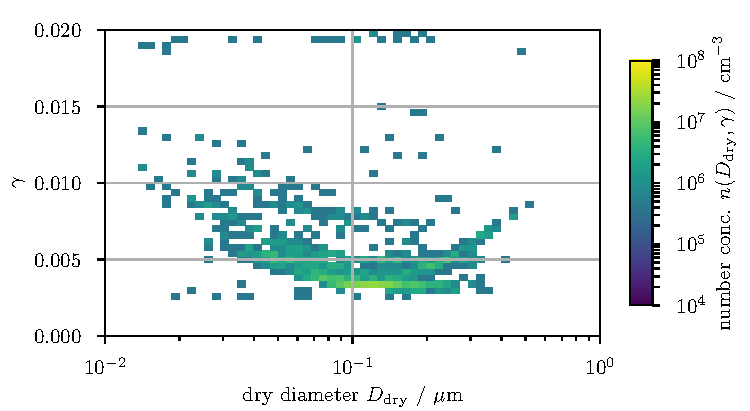
\includegraphics{urban_plume_diam_gamma_dist_00000012}
  \caption{2D histogram of $\gamma_i$, after 12 hour simulation of our
    ``urban plume'' case, using the parameterization according to
    Eq.~(\ref{eq:n2o5_param}). (Note: There is a lot of nitrate
    formation in this scenario, so many particles have a
    $\gamma$-value near 0.002.) \label{fig:2Dgamma}}
\end{figure}
However, evaluating Equation~\ref{eq:k} is rather complicated as one
needs to know the aerosol mixing state for a given aerosol. It would
be much more convenient to use an ``average $\gamma$'' based on the
bulk mass fractions, rather the per-particle mass fractions, like
this:
\begin{align} \label{eq:k_bulk}
  k^{\rm bulk}_{\rm N_2O_5} & = \frac{1}{4} c_{\rm  N_2O_5} S \gamma(\vec{\omega}_{\rm avg}), \\
  \text{with } \vec{\omega}_{\rm avg} & = \frac{1}{\sum_i m_i} \sum_i m_i \vec{\omega}_i,
\end{align}
where $\vec{\omega}_{\rm avg}$ are the bulk mass fractions (i.e.\ how
much sulfate and nitrate exists in the entire population). The
question arises: Is $k^{\rm bulk}_{\rm N_2O_5}$ in Eq.~\ref{eq:k_bulk}
equal to $k_{\rm N_2O_5}$ in Eq.~\ref{eq:k}? Short answer: No. Longer
answer:
\begin{align}
  \gamma(\vec{\omega}_{\rm avg}) & =  \vec{a}^{\rm T} \vec{\omega}_{\rm avg} \\
  \qquad &  = \vec{a}^{\rm T} \frac{1}{\sum_i m_i} \sum_i m_i \vec{\omega}_i \\
  \qquad & = \frac{1}{\sum_i m_i} \sum_i m_i \gamma_i
\end{align}

Use this in Eq.~\ref{eq:k_bulk}:
\begin{align}
  k^{\rm bulk}_{\rm N_2O_5} & = \frac{1}{4} c_{\rm  N_2O_5} S \frac{1}{\sum_i m_i} \sum_i m_i \gamma_i.
\end{align}
This is different to Eq.~\ref{eq:k}. Using the bulk mass fractions
overweights larger particles (should be surface-weighted, but is
mass-weighted). The error will be especially large, when $\gamma_i$ is
a function of size, i.e.\ larger particles have a different uptake
coefficient from smaller particles. For a monodisperse population
mixing state won't matter.


\begin{figure}
  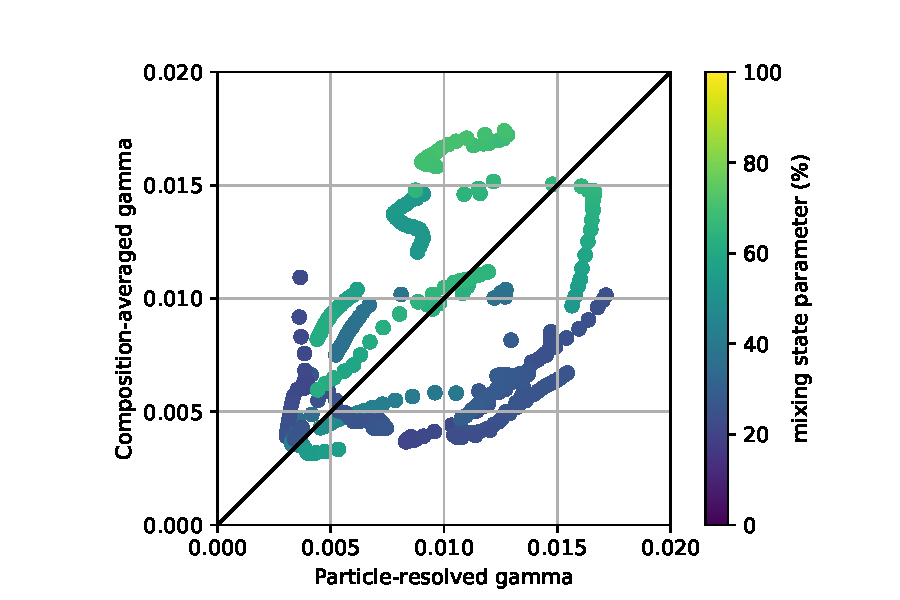
\includegraphics{gamma_values_20_scenarios}
\caption{$\gamma_{\rm N_2O_5}(\vec{\omega}_i)$ (based on per-particle composition) and
  $\gamma(\vec{\omega}_{\rm avg})$ (based on bulk composition) for 20
  scenarios. The points are coloured by the mixing state index
  $\chi$. \label{fig:gamma_values_20_scenarios}}
\end{figure}
Figure~\ref{fig:gamma_values_20_scenarios} shows how uptake
coefficients calculated based on per-particle composition compare to
the uptake coefficients calculated based on bulk composition. The
particle populations are output from a preliminary scenario library of
20 scenarios that vary in initial conditions and emissions. The uptake
coefficients for these simulations are calculated using a
parameterization that takes into account an organic coating around an
aqueous inorganic core. So the function is a bit more complicated than
Eq.~(\ref{eq:gamma_i}).

\section{Comparing results with and without the hydrolysis reaction}
I repeated the 20 scenarios but set the uptake coefficient to 0, hence
the hydrolysis reactions was ``switched off''. The graphs in
Figure~\ref{fig:scatter} compare the results of the two sets of
simulations for $\rm HNO_3$, $\rm O_3$ and nitrate. Each data point is
hourly output.

\begin{figure}
  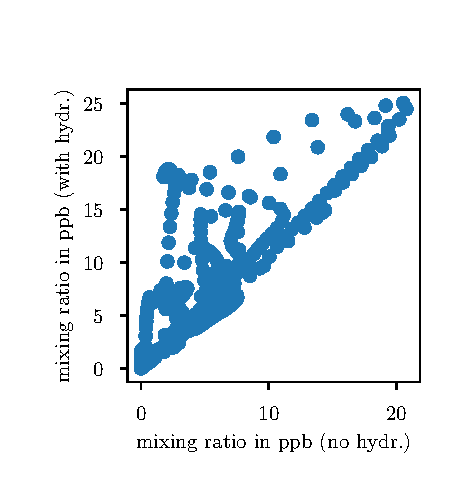
\includegraphics[scale=0.7]{scatter_hno3}
  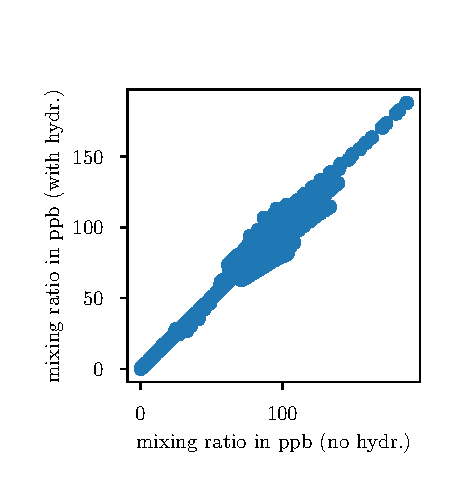
\includegraphics[scale=0.7]{scatter_o3}
  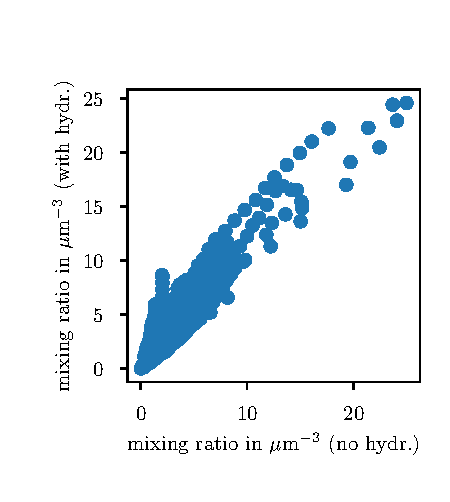
\includegraphics[scale=0.7]{scatter_no3}
    \caption{Comparison of results with and without hydrolysis for
      $\rm HNO_3$, $\rm O_3$ and nitrate. \label{fig:scatter}}
  \end{figure}

\clearpage \newpage
\bibliographystyle{plain-local-chicago} \bibliography{xxx}
\end{document}


